% !TEX root = Time_Evo.tex

\subsection{含时演化结果演示}
在量子力学中,量子系统的状态用波函数(wave function)来描述,在这里我们使用$\Psi(r,t)$表示被研究体系的总波函数,$r$是体系的位置,$t$为时间。求解含时薛定谔方程可以得到波函数随时间演化的所有信息,波函数是波动方程的解,具有类波的性质。需要注意,波函数$\Psi(r,t)$本身是复值函数,其值表示粒子在某一确定的时间空间点处的概率幅度;而波函数表达式的模平方${|\Psi(r,t)|}^2$表示在该时空点上粒子出现的概率,因此量子体系并不像经典力学体系那样具有确定性,它是建立在统计力学之上的。

为了将波函数概率分布变得可视化,我们将${|\Psi(r,t)|}^2$对空间坐标量对应作图。由于哈密顿量选取的是一维简谐振子模型,我们将初始的波函数设为一系列分立的振动能级本征波函数,求解薛定谔方程:
\begin{equation}
  -\frac{\hbar^2}{2\mu}\frac{d^2\Psi}{dx^2} + \frac{1}{2}kx^2\Psi = E \Psi
\end{equation}
\noindent 得到能量本征值为:
\begin{equation}
  E_{\nu} = \left( \nu + \frac{1}{2}\right ) h \nu_e
\end{equation}
\noindent 其中$\nu$为整数$0,1,2,\cdots$,相应的本征函数为:
\begin{equation}
  \Psi = N_{\nu}e^{-q^2/2}H_{\nu}(q)
\end{equation}
\noindent 其中$N_{\nu} = {\left[ \sqrt{b/\pi} / 2^{\nu} \nu ! \right]}^{1/2}$是归一化系数,$H_{\nu}$是厄米多项式,
\begin{equation}
  H_{\nu}(q) = \nu ! \sum_{k=0}^{\nu / 2} \left[ \frac{{(-1)}^k}{k! {(\nu - 2k)!}} \right] {(2q)}^{\nu-2k}
\end{equation}
可以得到如图\ref{fig:Psi_Fig}的线性谐振子能级、波函数和概率分布图。
\begin{figure}[h]
  \center
  \vspace{-1mm}
  \includegraphics[width=0.95\linewidth]{3.1/Psi_Fig.png}
  \caption{线性谐振子能级、波函数和概率分布图}
  \label{fig:Psi_Fig}
\end{figure}
正如\ref{sec:basis}所述,我们使用一系列$sinc$函数拟合谐振子的波函数。首先声明程序中使用的默认参数:全部使用原子单位(a.u.);采样点数为100并等距采样,采样空间为[-2,2];简谐振子的力常数$k=4{\pi}^2{\nu_e}^2\mu$中,令$\nu_e$和$\mu$均为1;含时演化的单位时间间隔$dt$定为0.01。

将$\Psi$用$sinc$函数展开后得到一个系数向量,在接下来的处理中这个向量将代替波函数的具体形式出现,即所有算符操作都是作用在系数向量上的。在构造含时演化算符$U(t) = e^{(-i/\hbar)\hat{H}t}$在希尔伯特空间中的表示矩阵后,每一步含时演化即将演化算符作用在系数矩阵上。将作用后的新系数向量归一化并做逆变换,就得到了单步演化后的波函数。由于我们采用间断演化,时间尺度上是不连续的,因此$dt$的取值越小则越接近真实的情况;由于原子单位中单位时间约为2.4$\times$10$^{-17}$s,可以认为我们的时间间隔足够小,能够大约模拟出含时演化的过程。

按照理论预测,我们构造的是一维简谐振子的哈密顿矩阵,当相应的含时演化算符作用在一维谐振子本征态的时候,应该预期得到不随时间变化的波函数;而当演化算符作用在非本征态时,波函数的空间概率分布将会发生变化。我们的计算机程序给出了这些过程的演化情况。
\begin{figure}[hbt]
  \centering
  \captionsetup{justification=centering}
  \vspace{1mm}
  \includegraphics[width=0.85\linewidth]{3.1/v=0}
  \includegraphics[width=0.85\linewidth]{3.1/v=1}
  \caption{简谐振子本征态含时演化 \\
            $\Psi = N_{\nu}e^{-q^2/2}H_{\nu}(q)$ \label{fig:prop1}}
\end{figure}

\begin{figure}[hbt]
  \centering
  \captionsetup{justification=centering}
  \vspace{1mm}
  \includegraphics[width=0.95\linewidth]{3.1/rand1}
  %\includegraphics[width=0.75\linewidth]{3.1/rand2}
  \caption{非本征态含时演化  \label{fig:prop2}}
\end{figure}

图\ref{fig:prop1}和图\ref{fig:prop2} 是使用切比雪夫展开进行的演化演示图,使用对角化方法可以得到类似的结果。我们发现,演化算符作用在本征态上时确实不会改变波函数的空间概率分布,而作用在非本征态上的结果有些难以预测。目前观察的结论是非本征态在短时间内会发生类周期性变化,波形不断改变。


\subsection{切比雪夫展开项数的影响}
首先我们考察最感兴趣的切比雪夫展开的变现。如图\ref{fig:prop1}所示,在本征态时切比雪夫展开的含时演化算符并不改变本征态的概率分布,符合预期。影响切比雪夫展开的参数因子有:格点数$N$,时间步长$dt$和切比雪夫展开项的数量$M$。接下来我们逐一讨论它们的影响。

正如之前所推导的,切比雪夫多项式展开是一个递归算法,$\Phi_{n+1}(\hat{X}) = 2\hat{X}\Phi_{n}(\hat{X}) + \Phi_{n-1}(\hat{X})$,显然展开项的数量对展开的精度有影响。可以预测,随着展开项数的增加,含时演化算符的表示矩阵中的元素会收敛于一定值,因此精度越来越高;然而也要注意每增加一项,计算机就要多进行一次递归循环,会增加占用的计算资源。因此我们希望找到合适的展开项数量。

由于切比雪夫展开本质上可以看做哈密顿算符线性变化得到的多项式,因此其作用在本征函数上,经归一化后理论上是不会发生变化的,也就是说改变展开项数量不会影响本征态。事实上我们的程序测试也证明了这一点。所以我们选用非本征态$\Psi(x) = \sqrt[4]{2}e^{-\pi x^2 /10}$作为研究对象,选择$dt=0.01$,格点数$N=100$为参数。将不同的展开项得到的结果与对角化我结果相比较(同时也和自身的变化趋势比较,观察其变化情况是否收敛),结果发现最佳的展开项数为40。
\begin{table}[!ht]
  \centering
  \begin{tabular}{P{2.2cm}|P{2.2cm}|P{2.2cm}}
    \hline
    \multicolumn{3}{c}{$\Psi(x) = \sqrt[4]{2}e^{-\pi x^2 /10}$}\\ \hline
     展开项数 & 波形 & 能量/a.u.  \\ \hline
     20 & 非正常 & 3.157                    \\ \hline
     25 & 非正常 & 19.666 \\ \hline
     30 & 非正常 & 8.376                    \\ \hline
     35 & 正常 & 15.082 \\ \hline
     40 & 正常  & 14.810                    \\ \hline
     45 & 正常 & 14.810 \\ \hline
     50 & 正常 & 14.810                  \\ \hline
     55 & 正常 & 14.810 \\ \hline
     60 & 正常 & 14.810                  \\ \hline
  \end{tabular}
\captionof{table}{\textbf{不同展开项数结果比较}}
\label{tab:num_expansion}
\end{table} \par 

\begin{figure}[h]
  \centering
  \captionsetup{justification=centering}
  \vspace{1mm}
  \includegraphics[width=0.95\linewidth]{3.2.1/M_num}
  \caption{不同展开项演化图示\\
            $\Psi(x) = \sqrt[4]{2}e^{-\pi x^2 /10}$  \label{fig:M_num}}
\end{figure}
上述的波形正常与否的判断主要依据两个判据:首先是和对角化方法给出的演化波函数的波形和能量对比,结果发现波形与对角化结果几乎一样,能量相近,约为14.810(a.u.);其次是和这一系列波函数自身的变化趋势比较,发现当$n \geq 40$时波函数的波形和能量都基本收敛。图\ref{fig:M_num}给出了6个时刻的演化波形。因此接下来程序中使用的切比雪夫展开项数默认情况下设置为40。有意思的是,当我们改变了其他默认参数(例如$dt$)时,40项切比雪夫展开可能就不足以准确近似含时演化算符,所以我们现在讨论的是上述默认参数情况下选用的最优展开项。改变时间步长对所需展开项数的影响将在后面分析。

\subsection{格点数$N$对切比雪夫展开的影响}
格点数$N$是我们在波函数采样区间$\left[-2,2\right]$内的采样点数,我们采用的是等距节点法。按照常识来说采样点越多那么计算的精度越高,不过更多的采样点也意味着需要更多计算资源。由于哈密顿量的表达式含有动量项,而动量算符涉及波函数的二阶求导,在我们使用的二阶差分方法中(公式\ref{eq:three-point} )两个相邻$x$的取值越接近则所做差分越准确。

由于切比雪夫展开和对角化方法都使用了$N$阶矩阵,我们可以将二者作相应的对比参照。如图\ref{fig:N_Cheby}和图\ref{fig:N_Diag}分别是切比雪夫展开和对角化方法以$dt=0.01$为步长演化100步得到的波函数。从波形和能量不难发现$N=50$的采样数过少,哈密顿量不够精确,演化得到的波函数和其他结果差别较大。有意思的是,当采样点数大于300时,切比雪夫方法出现了问题,波形与能量有很大偏差,后面会给出可能的原因。为了用合适的计算机资源得到足够准确的结果,我们将最优采样点数$N$选取为200。

\begin{figure}[h]
  \centering
  \captionsetup{justification=centering}
  \vspace{1mm}
  \includegraphics[width=0.95\linewidth]{3.2.2/N_Cheby}
  \caption{格点数对切比雪夫展开的影响 \label{fig:N_Cheby}}
\end{figure}
\begin{figure}[h]
  \centering
  \captionsetup{justification=centering}
  \vspace{1mm}
  \includegraphics[width=0.95\linewidth]{3.2.2/N_Diag}
  \caption{格点数对对角化方法的影响 \label{fig:N_Diag}}
\end{figure}

接下来讨论切比雪夫在$N$值过大时算法崩溃的可能原因。注意$\hat{H}_{norm}$的表达式$\hat{H}_{\text{norm}}  =  (\hat{H} - \hat{I}*H_{\text{half}}) / \Delta H$,只有$\hat{H}$的对角元素被减去$H_{half}$,非对角元素并没有被投影到[-1,1]区间上。在递归算法中每一步都要进行矩阵乘法运算,如果在$H$中含有较大的元素且在矩阵乘法中累积增大,那么最终有可能导致数据溢出。之前我们讨论过,利用三点近似法和局域近似法得到的哈密顿矩阵的本征值随着简谐振子能级的增长将加剧偏离理论值。也就是说,采样点数$N$值越大,哈密顿矩阵中最大的本征值对理论值得偏离越大。因此很可能在$N>300$后发生了数据溢出,经过归一化的错误演化波函数自然不符合预期。这里仅仅提出假设,今后的工作会进一步研究程序运行错误的原因。
\begin{figure}[hbt]
  \centering
  \captionsetup{justification=centering}
  \vspace{1mm}
  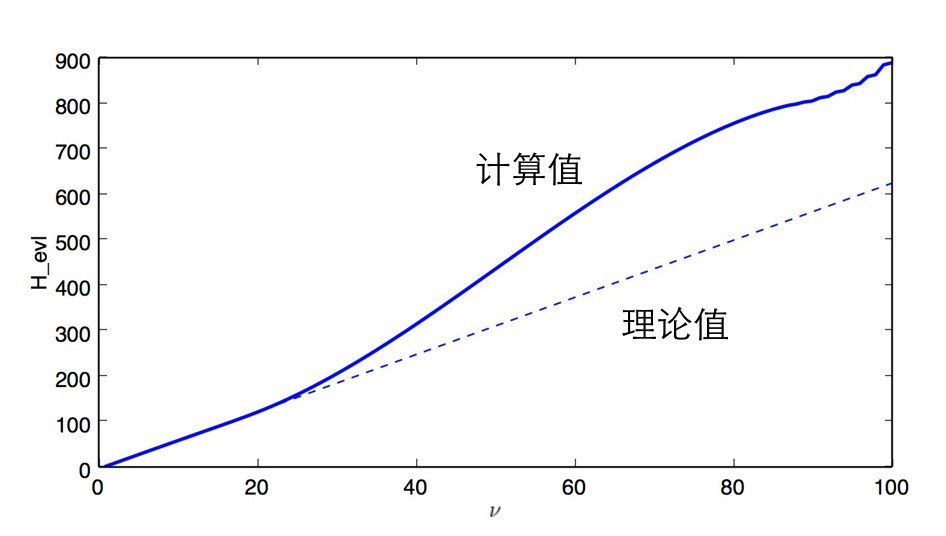
\includegraphics[width=0.9\linewidth]{H_err/H_err.jpg}
  \caption{哈密顿量本征值计算结果的偏差 \label{fig:N_Hamiltonian}}
\end{figure}


\subsection{演化时间步长的影响}
注意到图\ref{fig:N_Cheby}(f)的异常情况,笔者怀疑是切比雪夫展开的数值方法在程序运行时发生崩溃,考虑到还有参数$dt$可以共同调节切比雪夫展开项的大小,改变时间步长并研究切比雪夫展开的性质可能可以支持之前的猜想。

全局演化方法处理含时演化算符在数学上的可行性是显然的:
\begin{IEEEeqnarray}{rCl}
  \Psi(t_1 + t_2) & = & \hat{U}(t_1 + t_2) \Psi(0)\nonumber \\
  & = & e^{(-i/\hbar)\hat{H}(t_1 + t_2)} \Psi(0)\nonumber \\
  & = & e^{(-i/\hbar)\hat{H}t_1} e^{(-i/\hbar)\hat{H}t_2}\Psi(0)\nonumber \\
  & = & \hat{U}(t_1) \hat{U}(t_2) \Psi(0) 
\end{IEEEeqnarray}
因此可以根据所需要演化的时间直接确定$dt$的值。无论是单步长步长演化还是多步短步长演化理论上结果是一样的。

在我们的简单模型中,理论与计算结果都表明直接对角化方法处理含时演化算符是可行的,在这里我们暂时不考虑效率的问题。对角化方法唯一依赖的参数是采样点数$N$,只要我们得到了哈密顿量的矩阵表示,所有剩下的问题只是将这个厄米矩阵对角化并求出特征向量和特征值。大量测试数据表明,对角化方法的演化结果和多步短步长切比雪夫演化结果一致性较高,图\ref{fig:Diag_evo} 是对角化方法单步和多步演化的结果,其中$\Psi(x) = 2 \sqrt[4]{2\pi^2}x e^{-\pi x^2 /10}$,参数为$N=250$,多步法中$dt=0.01$演化10步,单步法中$dt=0.1$,展开项数为。因此在切比雪夫展开和对角化方法的对比中,我们认为对角化方法的结果是近似准确的,并以此优化切比雪夫展开的参数设定。

\begin{figure}[hbt]
  \centering
  \captionsetup{justification=centering}
  \vspace{-1mm}
  \includegraphics[width=0.99\linewidth]{3.3/Diag.pdf}
  \caption{对角化方法单步与多步演化结果 \\
            $\Psi(x) = 2 \sqrt[4]{2\pi^2}x e^{-\pi x^2 /10}$}
  \label{fig:Diag_evo}
\end{figure}

接下来我们尝试切比雪夫展开的单步和多步演化,发现了其中的问题。我们发现使用小步长多次演化的结果与对角化演化的结果一致,然而大步长单词演化的结果有偏差。也就是说,使用我们的切比雪夫展开,初始体系一次演化10个单位时间的结果和进行10次单步演化的结果不一样,这显然是有悖常理的。图\ref{fig:Cheby_evo} 显示了这一错误结果。
\begin{figure}[hbt]
  \centering
  \captionsetup{justification=centering}
  \vspace{-1mm}
  \includegraphics[width=0.99\linewidth]{3.3/Cheby.pdf}
  \caption{切比雪夫展开法单步与多步演化结果 \\
            $\Psi(x) = 2 \sqrt[4]{2\pi^2}x e^{-\pi x^2 /10}$}
  \label{fig:Cheby_evo}
\end{figure}
既然多步演化给出的计算结果与对角化方法结果一直,我们姑且认为切比雪夫展开的理论推导与模型建立是正确的,那么问题只能出现在数值计算的过程中了。笔者仔细查看了程序中含时演化算符表达式(公式\ref{eq:cheby_equation} ),其中涉及$dt$项的只有相位调节因子$\beta$和系数$a_n$,其他诸如切比雪夫递归项中不涉及$dt$,因此确定了寻找问题的切入点。
\begin{equation*}
  \Psi(t) \approx e^{\beta} \sum_{n=0}^{N} a_n \phi_n[-i H_{\text{norm}}] \Psi(0)
\end{equation*}
在确认贝塞尔函数和递归函数的程序编写无误后,问题的矛头指向了切比雪夫展开项数。通过增加展开项数量,单步演化的结果成功收敛于期望值。在尝试增加展开项数的过程中,我们还发现$dt$的正加似乎会剧烈影响达到收敛的展开项数,为此我们制作了$dt$-收敛展开项数关系表,见表\ref{tab:dt-M}和图\ref{fig:dt-M},其中收敛的标准定位能量值精确到6位有效数字。
\begin{table}[hbt]
  \centering
  \begin{tabular}{|P{3.5cm}|P{3.5cm}|}
    \hline
    \multicolumn{2}{|c|}{N=250}\\ \hline
    $dt$ & 所需展开项数  \\ \hline
    0.01 & 40                    \\ \hline
    0.02 & 70                    \\ \hline
    0.05 & 160                    \\ \hline
    0.1 & 290                  \\ \hline
    0.15 & 430         \\ \hline
    0.2 & 560                  \\ \hline
  \end{tabular}
\captionof{table}{\textbf{$\boldsymbol{dt}$-展开项数关系}}
\label{tab:dt-M}
\end{table}

\begin{figure}[hbt]
  \centering
  \captionsetup{justification=centering}
  \vspace{-1mm}
  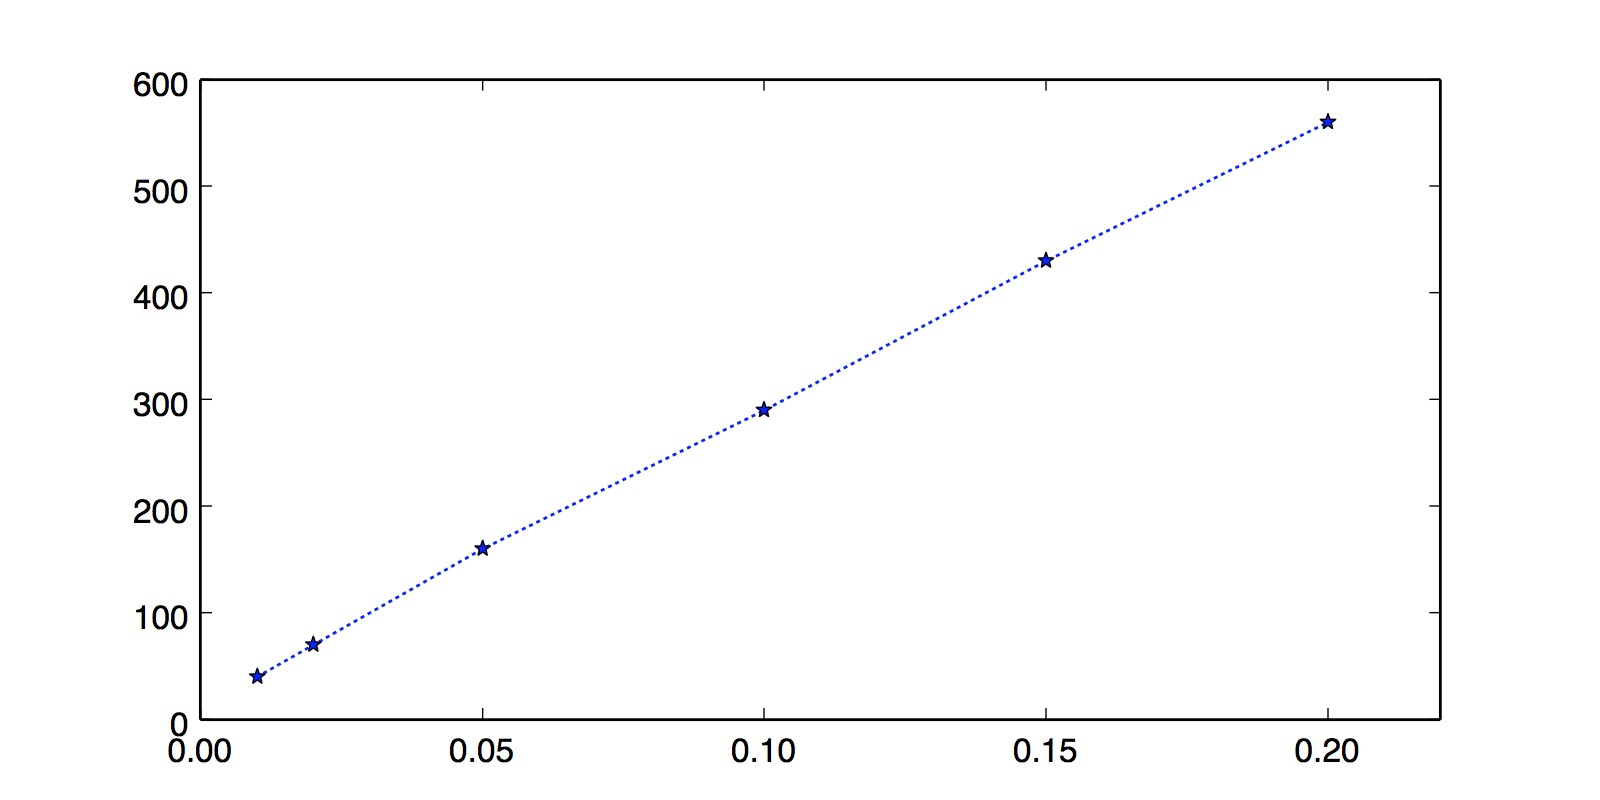
\includegraphics[width=0.99\linewidth]{dt-M/dt-M}
  \caption{$\boldsymbol{dt}$与展开项数关系}
  \label{fig:dt-M}
\end{figure}

可见随着时间步长的增长,所需要的切比雪夫多项式数量线性增长。我们手写的矩阵乘法的算法复杂度为$O(N^3)$,如果使用k步短步长演化,只需要将$\hat{U}$矩阵作用在波函数矢量上k次,即进行k次矩阵乘法;如果使用单步长步长演化,由于dt和展开项数的线性关系,相当于需要k倍的展开项系数才能构建$\hat{U}$,而每次递归循环中进行的复杂度最高的运算也是一次矩阵乘法,因此两种演化方法在复杂度上是相等的。

可以看出,在本课题所用模型中切比雪夫展开和对角化方法的表现较为一致。Blablabla...

\subsection{非本征态的含时演化} 